
%=============================================================================
\section{Multi-Threading in \DDG}
\label{sec:ddg4-multi-threading}
%=============================================================================
\subsection{Introductory Remarks}
\label{sec:ddg4-multi-threading-introduction}
%=============================================================================
\noindent
Multi-threading as supported by Geant4 is event driven. This means that 
the simulation of a given event is handled by one single thread.
Geant4 provides specific extensions to ease the users the use of its 
multi-threaded extensions~\cite{bib:Geant4-multi-threading}~\footnote{Please
note that the whole of Geant4 and your client code must be compiled with
the compile flag ${\tts{-DGEANT4_BUILD_MULTITHREADED=ON}}$}.
These extension divide in a formalized manner all actions to be performed
to setup a Geant4 multi-threaded program into

\begin{itemize}\itemcompact
\item {\bf{common}} actions to be performed and shared by all threads.
This includes the setup of the geometry and the physics list. The
other main area are
\item {\bf{thread-specific}} actions to be performed for each thread.
These are composed by the user actions called during the processing of
each run. These are the run-, event-, generation-, tracking-, 
stepping and stacking actions.
\end{itemize}

\noindent
To understand the interplay between \DDG and Geant4 let us quickly 
recapitulate the Geant4 mechanism how to configure multiple threads.
The setup of a multi-threaded application in Geant4 is centered around 
two additional classes, which both deal with single- and multi-threaded 
issues:

\begin{itemize}\itemcompact
\item {\tts{G4VUserActionInitialization}} class with 2 major callbacks:
	{\tts{Build()}} which is executed for each {\bf{worker thread}} and 
	{\tts{BuildForMaster()}} which is executed for master thread only.	
\item {\tts{G4VUserDetectorConstruction}} class with the callbacks
    {\tts{Construct()}}, where the shared geometry is constructed and
    {\tts{ConstructSDandField()}} where the sensitive detectors and the
    electro magnetic fields are provided.
\end{itemize}

\noindent
Both these Geant4 provided hooks are modeled in the standard \DDG 
way as action queues, which allow a modular and fine grained setup
as shown in Figure~\ref{fig:ddg4-user-initialization} and 
Figure~\ref{fig:ddg4-detector-initialization}.
\begin{figure}[t]
  \begin{center}
    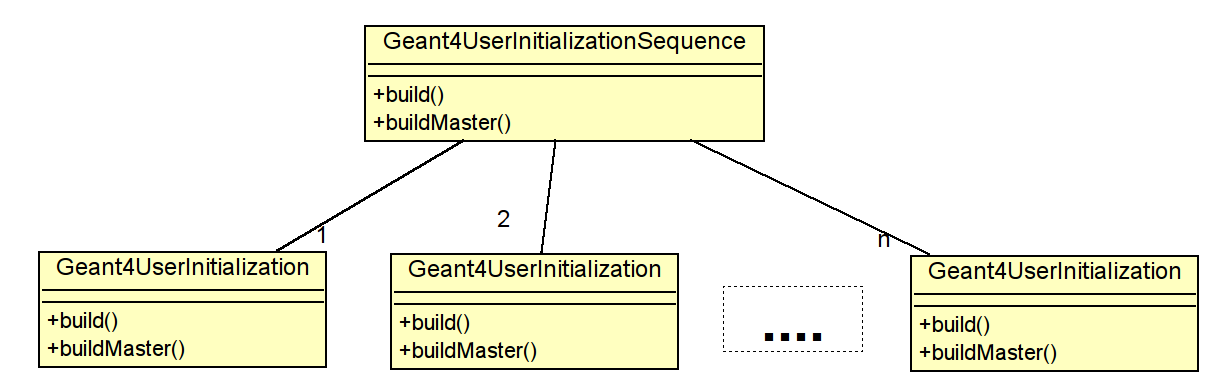
\includegraphics[width=140mm] {DDG4-User-Initialization.png}
    \caption{The Geant4 user initialization sequence to setup DDG4
             in multi-threaded mode. The callbacks {\tts{buildMaster()}} 
             is only called in multi-threaded mode.}
    \label{fig:ddg4-user-initialization}
  \end{center}
\end{figure}

\noindent
The \DDG framework ensures that all user callbacks are installed properly
to the Geant4 run manager, which calls them appropriately at the correct time.

\noindent
\DDG provides three callbacks for each sequence. Each callback receives
a temporary context argument, which may be used to shortcut access 
to basic useful quantities:
\begin{code}
    struct Geant4DetectorConstructionContext  {
      /// Reference to geometry object
      Geometry::LCDD&     lcdd;
      /// Reference to the world after construction
      G4VPhysicalVolume*  world;
      /// The cached geometry information
      Geant4GeometryInfo* geometry;
      /// G4 User detector initializer
      G4VUserDetectorConstruction* detector;
};
\end{code}

\begin{figure}[h]
  \begin{center}
    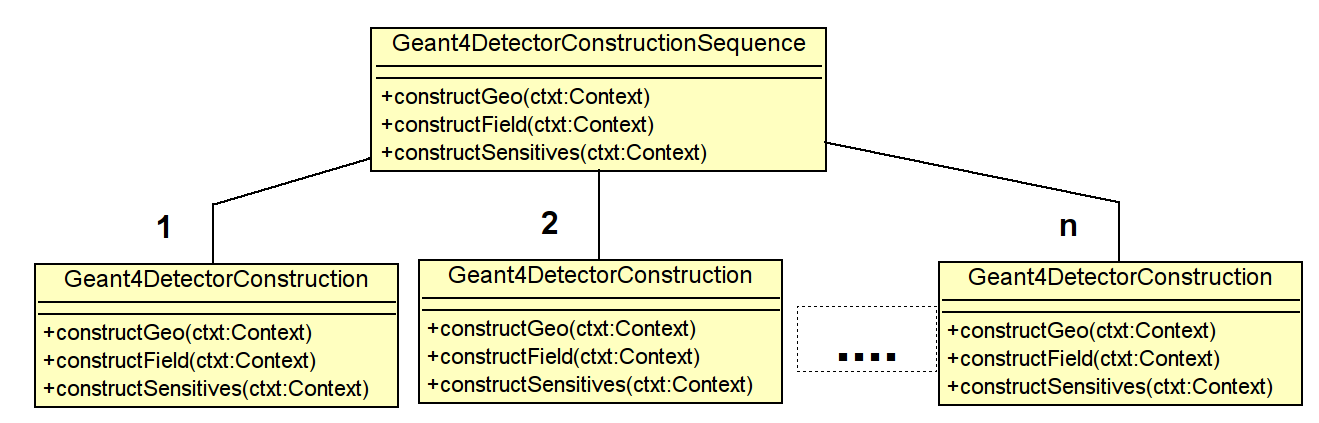
\includegraphics[width=140mm] {DDG4-Detector-Construction.png}
    \caption{The Geant4 detector initialization sequence to setup DDG4.
        If supplied, Geant4 calls the components both, in the single-threaded 
        and in the multi-threaded mode.}
    \label{fig:ddg4-detector-initialization}
  \end{center}
\end{figure}

The callbacks and the expected functionality are:
\begin{enumerate}
\item First the detector geometry is constructed. This happens in the callback
    {\tts{constructGeo(...)}}. If a standard \DDhep geometry 
    is present, this is translation of the geometry could be done by simply 
    calling the plugin {\tts{Geant4DetectorGeometryConstruction}}. 
    Alternatively a user defined plugin could perform this action.
\item Next the electromagnetic fields for the Geant4 particle tracking is
    constructed. A generic plugin {\tts{Geant4FieldTrackingConstruction}}
    may be attached. The corresponding setup parameters are listed in
    Section~\ref{sec:existing-ddg4-components}. 
    Alternatively a user defined plugin could perform this action.
\item Finally the Geant4 sensitive detectors are instantiated and attached 
    to the sensitive volumes. For generic setups the plugin
    {\tts{Geant4DetectorSensitivesConstruction}} may be attached.
    Alternatively a user defined plugin could perform this action.
\end{enumerate}

%=============================================================================
\subsection{Thread related contexts}
\label{sec:ddg4-thread-save context}
%=============================================================================
\noindent
\DDG provides thread related context, which may be accessed or modified
by user code. This context, the {\tts{Geant4Context}} and it's sub-components,
as discussed in Section~\ref{sec:ddg4-implementation-higher-level-components}
are available as separate instances for each event and as such
also independently for each worker thread. Hence, no user level locking of the 
event context is necessary in any worker thread.

%=============================================================================
\subsection{Thread-Shared Components}
\label{sec:ddg4-multi-threaded-shared-actions}
%=============================================================================
\noindent
Some actions, though executed in the context of a single thread context 
may only execute as singletons. An example would be a {\tts{GeneratorAction}},
which read input events from file. Clearly the reading of data from
file must be protected and the reading of one event in a given thread
must finish, before the next thread may take over.
Another example are data analysis components, which e.g. fill a histogram.
Typically the filling mechanism of a histogram is not thread safe and hence must
be protected.

\noindent
To solve such issues all actions, which may involve such shared 
activities, a shared action is provided, which adopts a singleton
instance and executes the relevant callbacks in a protected manner.
The shared actions execute the user component in a thread safe envelope.

\noindent
Clearly no run- or event related state in such shared actions may be
carried by the component object across callbacks. The action objects
may not be aware of the event related context outside the callback.
Default implementations for such shared actions exist for
\begin{itemize}\itemcompact
\item the {\tts{Geant4RunAction}}, where the calls to 
        {\tts{Geant4RunAction::begin}} and {\tts{Geant4RunAction::end}}
        are {\bf{globally}} locked and the sequential execution of 
        the entire sequence is ensured;
\item the {\tts{Geant4EventAction}},
\item the {\tts{Geant4TrackingAction}},
\item the {\tts{Geant4SteppingAction}} and
\item the {\tts{Geant4StackingAction}}.
\end{itemize}
In the latter cases the framework ensures thread safety, but does 
not ensure the reentrant execution order of the entire sequence.

\noindent
{\bf{General Remark:}}
\noindent
Simple callbacks registered to the run-, event, etc.-actions cannot 
be protected. These callbacks may under no circumstances use any 
event related state information of the called object.

%=============================================================================
\subsection{Backwards- and Single-Thread-Compatibility}
\label{sec:ddg4-multi-threading-backwards}
%=============================================================================
\noindent
As in the single threaded mode of Geant4, also in the multi-threaded
mode all user actions are called by an instance of the {\tts{G4RunManager}}
or a sublass thereof, the {\tts{G4MTRunManager}}~\cite{bib:Geant4-multi-threading}.

\noindent
If the recommended actions in sub-section~\ref{sec:ddg4-multi-threading-introduction}
are used to configure the Geant4 application, then in a rather transparent
way both single-threaded and multi-threaded setups can coexist simply by 
changing the concrete instance of the {\tts{G4RunManager}}. There is one
single exception: The user initialization function
{\tts{G4VUserActionInitialization::BuildForMaster()}} is {\bf{only}} executed
in multi-threaded mode. For this reason, we deprecate the usage. Try
to find solutions, without master specific setup using e.g. shared actions.

%=============================================================================
\subsection{Support for Python Setup in Multi-Threading Mode}
\label{sec:ddg4-multi-threading-python}
%=============================================================================
\noindent
The setup of \DDG in multi-threaded mode requires separate callbacks for 
the global configuration (geometry, etc.) and the configuration of the worker 
threads. In python this setup is performed within {\rm{python callable}}
objects, which are either functions or member functions of objects.
These functions may have arguments. The python specific configuration actions
\begin{itemize}\itemcompact
\item The user initialization action 
    {\tts{Geant4PythonInitialization}} allows to configure python callbacks
    for the master and the worker thread setup using the calls:
    \begin{code}
      /// Set the Detector initialization command
      void setMasterSetup(PyObject* callable, PyObject* args);
      /// Set the field initialization command
      void setWorkerSetup(PyObject* callable, PyObject* args);              \end{code}
     to be used in python as a call sequence within the master thread:
    \begin{code}
     init_seq = kernel.userInitialization(True)
     init_action = UserInitialization(kernel,'Geant4PythonInitialization/PyG4Init')
     init_action.setWorkerSetup(worker_setup_call, < worker_args > )
     init_action.setMasterSetup(master_setup_call, < master_args > )
     init_seq.adopt(init_action)                                            \end{code}
    The callback argument list $< worker\_args >$ and $< master\_args >$
    are python tuples containing all arguments expected by the callable objects
    $worker\_setup\_call$ and $master\_setup\_call$ respecyively.
    The class {\tts{Geant4PythonInitialization}} is a subclass of
    {\tts{Geant4UserInitialization}} and will call the provided functions
    according to the protocol explained earlier in this section.
    If a callback is not set, the corresponding actiion is not executed.
\item The detector construction action 
    {\tts{Geant4PythonDetectorConstruction}} is the corresponding 
    python action to populate the detector construction sequencer.
    and supports three ccallbacks:
    \begin{code}
      /// Set the Detector initialization command
      void setConstructGeo(PyObject* callable, PyObject* args);
      /// Set the field initialization command
      void setConstructField(PyObject* callable, PyObject* args);
      /// Set the sensitive detector initialization command
      void setConstructSensitives(PyObject* callable, PyObject* args);    \end{code}
    to be used in python as call sequence within the master thread:
    \begin{code}
    init_seq = self.master().detectorConstruction(True)
    init_action = DetectorConstruction(self.master(),name_type)
    init_action.setConstructGeo(geometry_setup_call, < geometry_args > )
    init_action.setConstructField(field_setup_call, < field_args > )
    init_action.setConstructSensitives(sensitives_setup_call, < sensitives_args >)
    init_seq.adopt(init_action)                                           \end{code}
    If any of the three callback is not set, the corresponding actiion is not executed.
    Hereby are $geometry\_setup\_call$, $field\_setup\_call$ and $sensitives\_setup\_call$ 
    the callable objects to configure the geometry, the tracking field 
    and the sensitive detectors.
    $< geometry\_args >$, $< field\_args >$ and $< sensitives\_args >$ are 
    the corresponding callable arguments in the form of a python tuple object.   
\end{itemize}

\noindent
All python callbacks are supposed to return the integer '1' on success.
Any other return code is assumed to be failure.

%=============================================================================
\subsection{\DDG Multi-Threading Example}
\label{sec:ddg4-multi-threading-example}
%=============================================================================
\begin{code}
"""

   DD4hep simulation example setup DDG4
   in multi-threaded mode using the python configuration

   @author  M.Frank
   @version 1.0

"""
import os, time, DDG4

def setupWorker(geant4):
  kernel = geant4.kernel()
  print '#PYTHON: +++ Creating Geant4 worker thread ....'
  print "#PYTHON:  Configure Run actions"
  run1 = DDG4.RunAction(kernel,'Geant4TestRunAction/RunInit')
    ...
  print "#PYTHON:  Configure Event actions"
  prt = DDG4.EventAction(kernel,'Geant4ParticlePrint/ParticlePrint')
  kernel.eventAction().adopt(prt)
    ...
  print "\n#PYTHON:  Configure I/O\n"
  evt_root = geant4.setupROOTOutput('RootOutput','CLICSiD_'+time.strftime('%Y-%m-%d_%H-%M'))
    ...
  gen = DDG4.GeneratorAction(kernel,"Geant4GeneratorActionInit/GenerationInit")
  kernel.generatorAction().adopt(gen)
  print "#PYTHON:  First particle generator: pi+"
  gen = DDG4.GeneratorAction(kernel,"Geant4IsotropeGenerator/IsotropPi+");
    ...
  print "#PYTHON:  Merge all existing interaction records"
  gen = DDG4.GeneratorAction(kernel,"Geant4InteractionMerger/InteractionMerger")
  kernel.generatorAction().adopt(gen)
  print "#PYTHON:  Finally generate Geant4 primaries"
  gen = DDG4.GeneratorAction(kernel,"Geant4PrimaryHandler/PrimaryHandler")
  kernel.generatorAction().adopt(gen)
  print "#PYTHON:  ....and handle the simulation particles."
  part = DDG4.GeneratorAction(kernel,"Geant4ParticleHandler/ParticleHandler")
  kernel.generatorAction().adopt(part)

  user = DDG4.Action(kernel,"Geant4TCUserParticleHandler/UserParticleHandler")
    ...
  part.adopt(user)
  print '#PYTHON: +++ Geant4 worker thread configured successfully....'
  return 1
  
def setupMaster(geant4):
  kernel = geant4.master()
  print '#PYTHON: +++ Setting up master thread for ',kernel.NumberOfThreads,' workers.'
  return 1

def setupSensitives(geant4):
  print "#PYTHON:  Setting up all sensitive detectors"
  geant4.printDetectors()
  print "#PYTHON:  First the tracking detectors"
  seq,act = geant4.setupTracker('SiVertexBarrel')
    ...
  print "#PYTHON:  Now setup the calorimeters"
  seq,act = geant4.setupCalorimeter('EcalBarrel')
    ...
  return 1

def run():
  kernel = DDG4.Kernel()
  lcdd = kernel.lcdd()
  install_dir = os.environ['DD4hepINSTALL']
  DDG4.Core.setPrintFormat("%-32s %6s %s")
  kernel.loadGeometry("file:"+install_dir+"/DDDetectors/compact/SiD.xml")
  DDG4.importConstants(lcdd)

  kernel.NumberOfThreads = 3
  geant4 = DDG4.Geant4(kernel,tracker='Geant4TrackerCombineAction')
  print "#  Configure UI"
  geant4.setupCshUI()

  print "#  Geant4 user initialization action"
  geant4.addUserInitialization(worker=setupWorker, worker_args=(geant4,),
                               master=setupMaster,master_args=(geant4,))
  print "#  Configure G4 geometry setup"
  seq,act = geant4.addDetectorConstruction("Geant4DetectorGeometryConstruction/ConstructGeo")

  print "# Configure G4 sensitive detectors: python setup callback"
  seq,act = geant4.addDetectorConstruction("Geant4PythonDetectorConstruction/SetupSD",
                                           sensitives=setupSensitives,sensitives_args=(geant4,))
  print "# Configure G4 sensitive detectors: atach'em to the sensitive volumes"
  seq,act = geant4.addDetectorConstruction("Geant4DetectorSensitivesConstruction/ConstructSD")

  print "#  Configure G4 magnetic field tracking"
  seq,field = geant4.addDetectorConstruction("Geant4FieldTrackingConstruction/MagFieldTrackingSetup")
  field.stepper            = "HelixGeant4Runge"
  field.equation           = "Mag_UsualEqRhs"
  field.eps_min            = 5e-05 * mm
  ...
  print "#  Setup random generator"
  rndm = DDG4.Action(kernel,'Geant4Random/Random')
  rndm.Seed = 987654321
  rndm.initialize()
  print "#  Now build the physics list:"
  phys = geant4.setupPhysics('QGSP_BERT')
  geant4.run()

if __name__ == "__main__":
  run()
\end{code}

\newpage